% Ensure that you compile using XeLaTeX !!! PDFTex has problems with some of the packages used
\documentclass[12pt]{article}
\setlength\parindent{0pt}

\usepackage{parskip}
\usepackage[margin=0.5in]{geometry}
\usepackage{fullpage}
\usepackage{moresize}
\usepackage{graphicx}
\usepackage{caption}
\usepackage{subcaption}
\usepackage{float}
\usepackage{xcolor}
\usepackage{soul}
\usepackage{fontspec}
\setmainfont{Doulos SIL}

\begin{document}

\begin{center}
\textbf{{\color{violet}{\HUGE 20201118 Wednesday\\}}}

\textbf{{\color{violet}{\HUGE ALL EXAMS\\}}}

\end{center}
\newpage

\begin{center}
\textbf{{\color{blue}{\HUGE START OF EXAM\\}}}

\textbf{{\color{blue}{\HUGE Student ID: 61058\\}}}

\textbf{{\color{blue}{\HUGE 9:00\\}}}

\end{center}
\newpage

{\large Question 1}\\

Topic: Acoustics\\
Source: Week 9 Handout, Question 7\\

Explain why each numbered, underlined statement is true or false. If it is false, explain one way that you could correct it.\\

Sound is a particular kind of wave known as a compression wave.... $^6$\ul{When the molecules are really close together, they try to spread out as far as possible, and that’s why they move out as a wave.}\\\\There are several key components of a sound wave. The first is wavelength. $^7$\ul{Wavelength is the distance between the point of maximum rarefaction and the point of maximum compression in a wave.} Another component that is related to wavelength is $^8$\ul{frequency, or how many times a wave passes through a particular point in one second.} $^9$\ul{If the wavelength is really short, the frequency will be really high; if the wavelength is really long, the frequency will be really low.} 


\newpage

{\large Question 2}\\

Topic: Phonological Features\\
Source: Quiz 3, Question 12\\

Explain how you figure out which feature is involved in the process of umlaut shown below.\\

\begin{figure}[H]
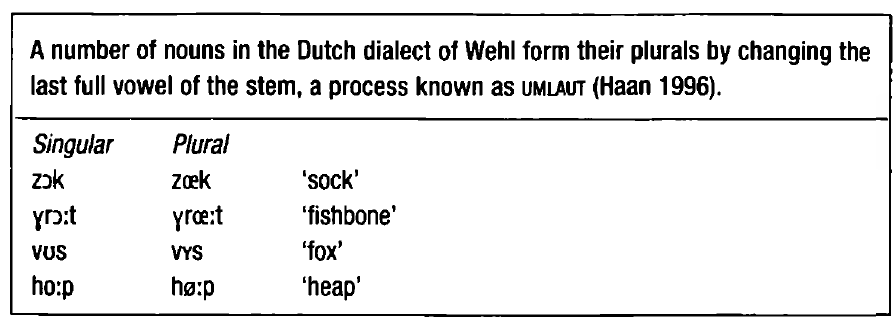
\includegraphics{../images/dutch.png}
\end{figure}

\newpage

\begin{center}
\textbf{{\color{red}{\HUGE END OF EXAM}}}\\

\end{center}
\newpage

\begin{center}
\textbf{{\color{blue}{\HUGE START OF EXAM\\}}}

\textbf{{\color{blue}{\HUGE Student ID: 49816\\}}}

\textbf{{\color{blue}{\HUGE 9:10\\}}}

\end{center}
\newpage

{\large Question 1}\\

Topic: Articulatory Phonetics\\
Source: Week 3 Handout, Question 13\\

Explain why this image does or does not match the description.\\

\begin{itemize} \item A one-handed sign. \item Location: At the signer’s nose. \item Handshape: Starts with index and middle finger crossed; the two fingers separate during the sign. \item Movement: No movement other than the change in handshape. \end{itemize}

\begin{figure}[H]
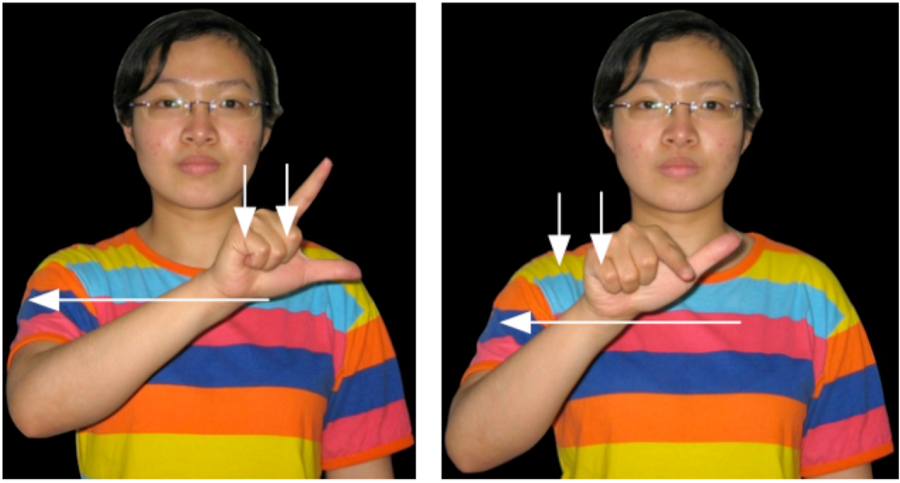
\includegraphics{../images/taiwansign_thing.png}
\caption{THING}
\end{figure}

\newpage

{\large Question 2}\\

Topic: Acoustics\\
Source: Week 9 Handout, Question 3\\

Explain what you see in the spectrogram that tells you about the properties of the sounds in the pictured word.\\

\begin{figure}[H]
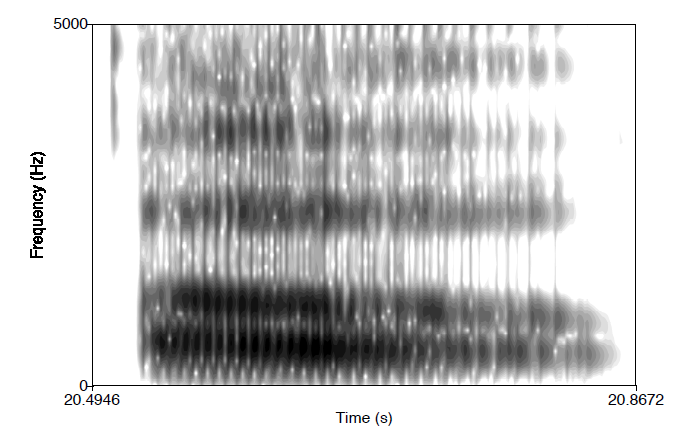
\includegraphics{../images/spectrogram_oh.png}
\end{figure}

\newpage

\begin{center}
\textbf{{\color{red}{\HUGE END OF EXAM}}}\\

\end{center}
\newpage

\begin{center}
\textbf{{\color{blue}{\HUGE START OF EXAM\\}}}

\textbf{{\color{blue}{\HUGE Student ID: 33428\\}}}

\textbf{{\color{blue}{\HUGE 9:20\\}}}

\end{center}
\newpage

{\large Question 1}\\

Topic: Acoustics\\
Source: Week 9 Handout, Question 7\\

Explain why each numbered, underlined statement is true or false. If it is false, explain one way that you could correct it.\\

Sound is an invisible phenomenon. Sound can travel through any substance, $^1$\ul{such as a liquid, solid, or a gas.} $^2$\ul{It involves the transfer of the matter in that substance} from one place to another.\\\\Sound is a particular kind of wave known as $^3$\ul{a compression wave}. $^4$\ul{When the molecules are really close together, we say they are ``rarefied'' and when they are really far apart, we say they are ``compressed.''}


\newpage

{\large Question 2}\\

Topic: Articulatory Phonetics\\
Source: Homework 1, Question 3(a)\\

Could this image be the result of producing the sound represented by the given IPA symbol? Why or why not?\\

{[ɾ]}

\begin{figure}[H]
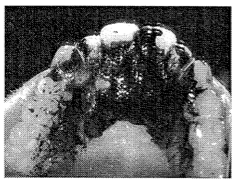
\includegraphics{../images/staticpalatography_stop.png}
\end{figure}

\newpage

\begin{center}
\textbf{{\color{red}{\HUGE END OF EXAM}}}\\

\end{center}
\newpage

\begin{center}
\textbf{{\color{blue}{\HUGE START OF EXAM\\}}}

\textbf{{\color{blue}{\HUGE Student ID: 56051\\}}}

\textbf{{\color{blue}{\HUGE 9:30\\}}}

\end{center}
\newpage

{\large Question 1}\\

Topic: Articulatory Phonetics\\
Source: Homework 1, Question 3(a)\\

Could this image be the result of producing the sound represented by the given IPA symbol? Why or why not?\\

{[z]}

\begin{figure}[H]
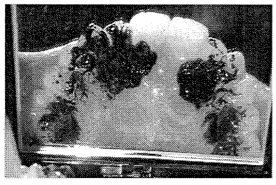
\includegraphics{../images/staticpalatography_fricative.png}
\end{figure}

\newpage

{\large Question 2}\\

Topic: Skewed Distributions\\
Source: Week 5 Handout, Question 1\\

Explain why we think that languages are not random in terms of their phonology.\\


\newpage

\begin{center}
\textbf{{\color{red}{\HUGE END OF EXAM}}}\\

\end{center}
\newpage

\begin{center}
\textbf{{\color{blue}{\HUGE START OF EXAM\\}}}

\textbf{{\color{blue}{\HUGE Student ID: 35405\\}}}

\textbf{{\color{blue}{\HUGE 9:40\\}}}

\end{center}
\newpage

{\large Question 1}\\

Topic: Phonological Features\\
Source: Week 4 Discussion\\

Explain what the given feature’s value is for this class of sounds, and why.\\

{[consonantal]}

glides


\newpage

{\large Question 2}\\

Topic: Other (pre-midterm)\\
Source: Week 5 \& 6 Handouts\\

Explain how you could analyze this dataset in terms of sequential patterns vs. paradigmatic patterns.\\

\begin{figure}[H]
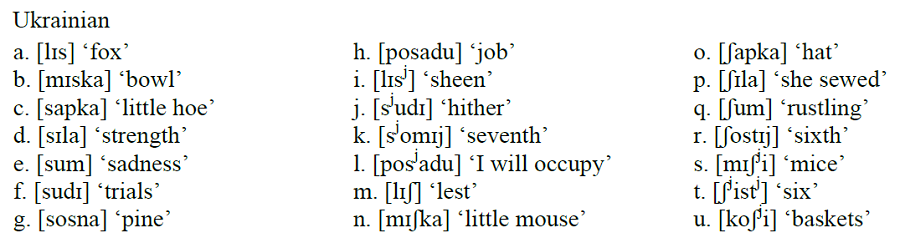
\includegraphics{../images/ukrainian.png}
\end{figure}

\newpage

\begin{center}
\textbf{{\color{red}{\HUGE END OF EXAM}}}\\

\end{center}
\newpage

\begin{center}
\textbf{{\color{blue}{\HUGE START OF EXAM\\}}}

\textbf{{\color{blue}{\HUGE Student ID: 34236\\}}}

\textbf{{\color{blue}{\HUGE 9:50\\}}}

\end{center}
\newpage

{\large Question 1}\\

Topic: Transcription\\
Source: Week 2 Handout, Part II, Question 11\\

How would this word be transcribed?\\ (Kathleen will then ask a follow-up question about your transcription.)\\

<goat>


\newpage

{\large Question 2}\\

Topic: Skewed Distributions\\
Source: Week 5 Handout, Question 6\\

If I gave you a new word in Malto, [di\_\_u], would it be possible to predict whether it's [d] or [t] that goes in the blank? Explain why or why not.\\

\begin{figure}[H]
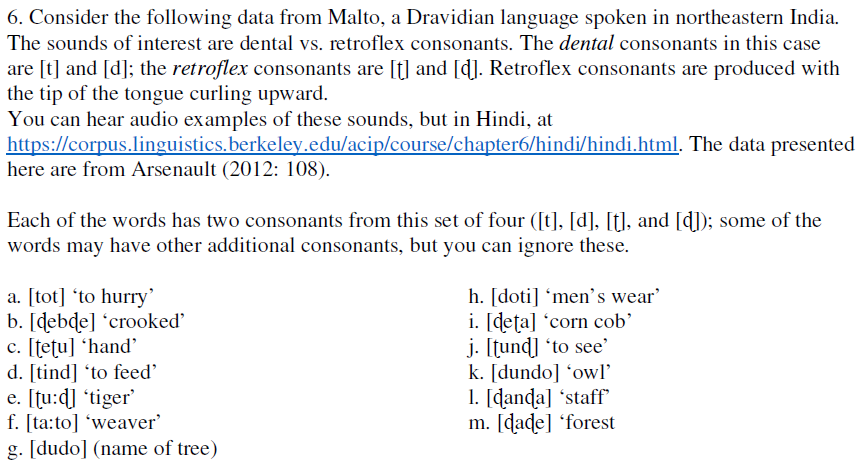
\includegraphics{../images/malto.png}
\end{figure}

\newpage

\begin{center}
\textbf{{\color{red}{\HUGE END OF EXAM}}}\\

\end{center}
\newpage

\begin{center}
\textbf{{\color{blue}{\HUGE START OF EXAM\\}}}

\textbf{{\color{blue}{\HUGE Student ID: 40922\\}}}

\textbf{{\color{blue}{\HUGE 4:00\\}}}

\end{center}
\newpage

{\large Question 1}\\

Topic: Articulatory Phonetics\\
Source: Week 3 Handout, Question 13\\

Explain why this image does or does not match the description.\\

\begin{itemize} \item A one-handed sign. \item Location: At the signer’s nose. \item Handshape: Starts with index and middle finger crossed; the two fingers separate during the sign. \item Movement: No movement other than the change in handshape. \end{itemize}

\begin{figure}[H]
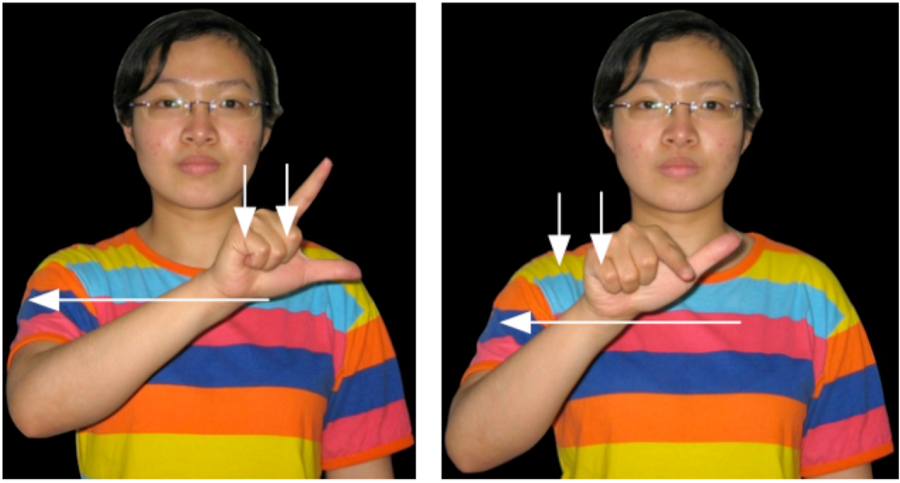
\includegraphics{../images/taiwansign_thing.png}
\caption{THING}
\end{figure}

\newpage

{\large Question 2}\\

Topic: Phonological Features\\
Source: Quiz 3, Question 12\\

Explain how you figure out which feature is involved in the process of umlaut shown below.\\

\begin{figure}[H]
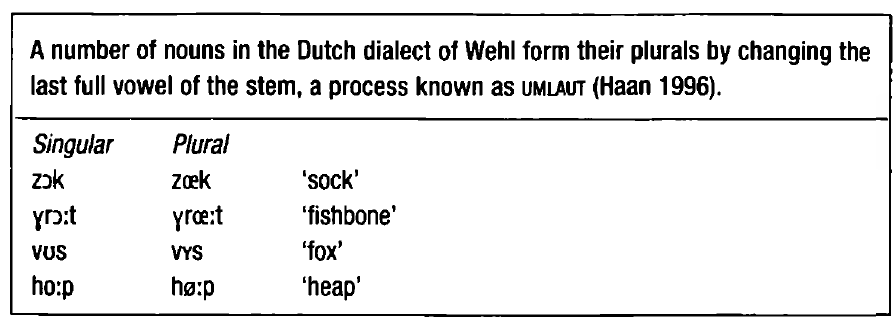
\includegraphics{../images/dutch.png}
\end{figure}

\newpage

\begin{center}
\textbf{{\color{red}{\HUGE END OF EXAM}}}\\

\end{center}
\newpage

\begin{center}
\textbf{{\color{blue}{\HUGE START OF EXAM\\}}}

\textbf{{\color{blue}{\HUGE Student ID: 48894\\}}}

\textbf{{\color{blue}{\HUGE 4:10\\}}}

\end{center}
\newpage

{\large Question 1}\\

Topic: Acoustics\\
Source: Week 9 Handout, Question 3\\

Explain what you see in the spectrogram that tells you about the properties of the sounds in the pictured word.\\

\begin{figure}[H]
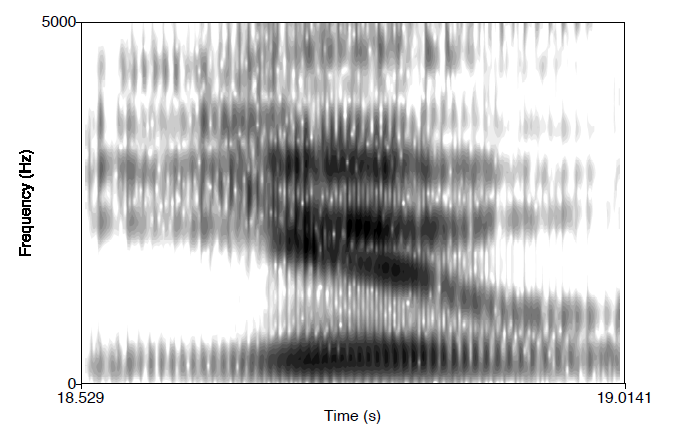
\includegraphics{../images/spectrogram_you.png}
\end{figure}

\newpage

{\large Question 2}\\

Topic: Other (pre-midterm)\\
Source: Week 4 Handout, Part II, Question 3\\

Explain how you would figure out what the Luiseño form is for the morpheme whose meaning is given below. (To be clear: you do NOT need to give me the form itself -- just explain the process of figuring it out.)\\

‘walk’

\begin{figure}[H]
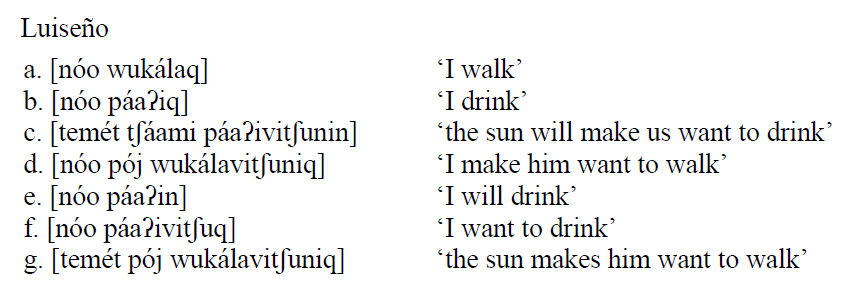
\includegraphics{../images/luiseno.png}
\end{figure}

\newpage

\begin{center}
\textbf{{\color{red}{\HUGE END OF EXAM}}}\\

\end{center}
\newpage

\begin{center}
\textbf{{\color{blue}{\HUGE START OF EXAM\\}}}

\textbf{{\color{blue}{\HUGE Student ID: 98910\\}}}

\textbf{{\color{blue}{\HUGE 4:20\\}}}

\end{center}
\newpage

{\large Question 1}\\

Topic: Skewed Distributions\\
Source: Week 5 Handout, Question 7\\

Explain how you would go about looking for co-occurrence restrictions in bi-syllabic signs in ASL. (Refer to the data that follows.)\\

\begin{figure}[H]
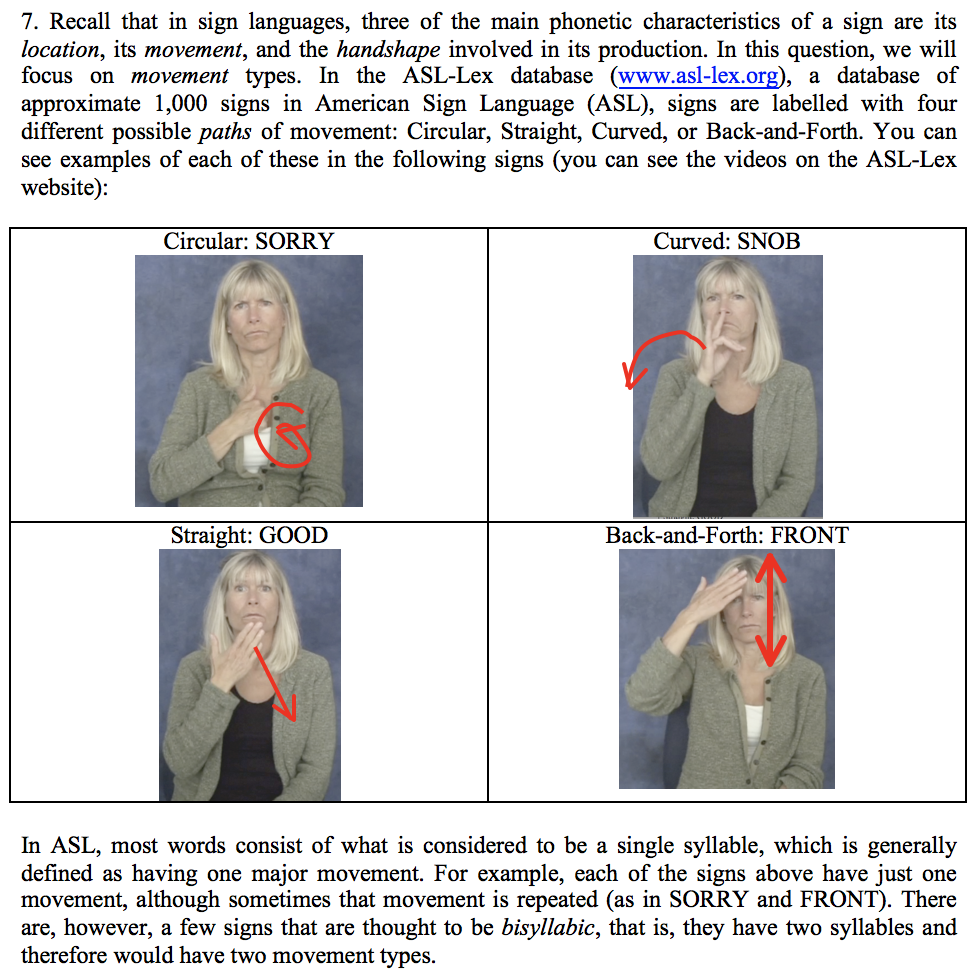
\includegraphics{../images/ASL_movement.png}
\end{figure}

\newpage

{\large Question 2}\\

Topic: Articulatory Phonetics\\
Source: Homework 1, Question 3(b)\\

Explain why this is or is not a complete phonetic natural class in standard North American English.\\

{[i]}, {[u]}, {[eɪ]}


\newpage

\begin{center}
\textbf{{\color{red}{\HUGE END OF EXAM}}}\\

\end{center}
\newpage

\begin{center}
\textbf{{\color{blue}{\HUGE START OF EXAM\\}}}

\textbf{{\color{blue}{\HUGE Student ID: 56149\\}}}

\textbf{{\color{blue}{\HUGE 4:30\\}}}

\end{center}
\newpage

{\large Question 1}\\

Topic: Articulatory Phonetics\\
Source: Homework 1, Question 3(a)\\

Could this image be the result of producing the sound represented by the given IPA symbol? Why or why not?\\

{[t͡ʃ]}

\begin{figure}[H]
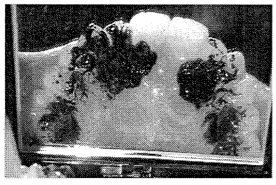
\includegraphics{../images/staticpalatography_fricative.png}
\end{figure}

\newpage

{\large Question 2}\\

Topic: Other (pre-midterm)\\
Source: Week 4 Handout, Part II, Question 3\\

Explain how you would figure out what the Luiseño form is for the morpheme whose meaning is given below. (To be clear: you do NOT need to give me the form itself -- just explain the process of figuring it out.)\\

‘walk’

\begin{figure}[H]
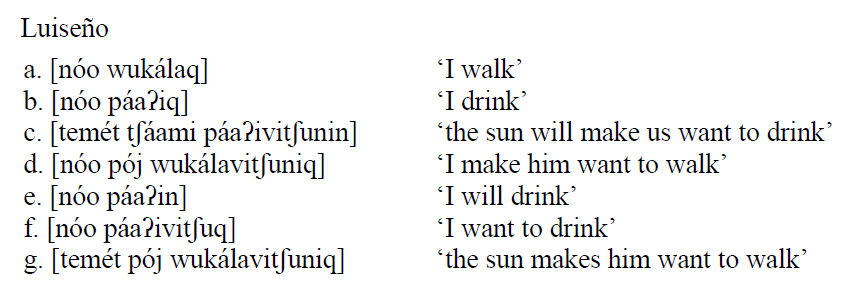
\includegraphics{../images/luiseno.png}
\end{figure}

\newpage

\begin{center}
\textbf{{\color{red}{\HUGE END OF EXAM}}}\\

\end{center}
\newpage

\begin{center}
\textbf{{\color{blue}{\HUGE START OF EXAM\\}}}

\textbf{{\color{blue}{\HUGE Student ID: 41381\\}}}

\textbf{{\color{blue}{\HUGE 4:40\\}}}

\end{center}
\newpage

{\large Question 1}\\

Topic: Skewed Distributions\\
Source: Week 5 Handout, Question 7\\

Explain how you would go about looking for co-occurrence restrictions in bi-syllabic signs in ASL. (Refer to the data that follows.)\\

\begin{figure}[H]
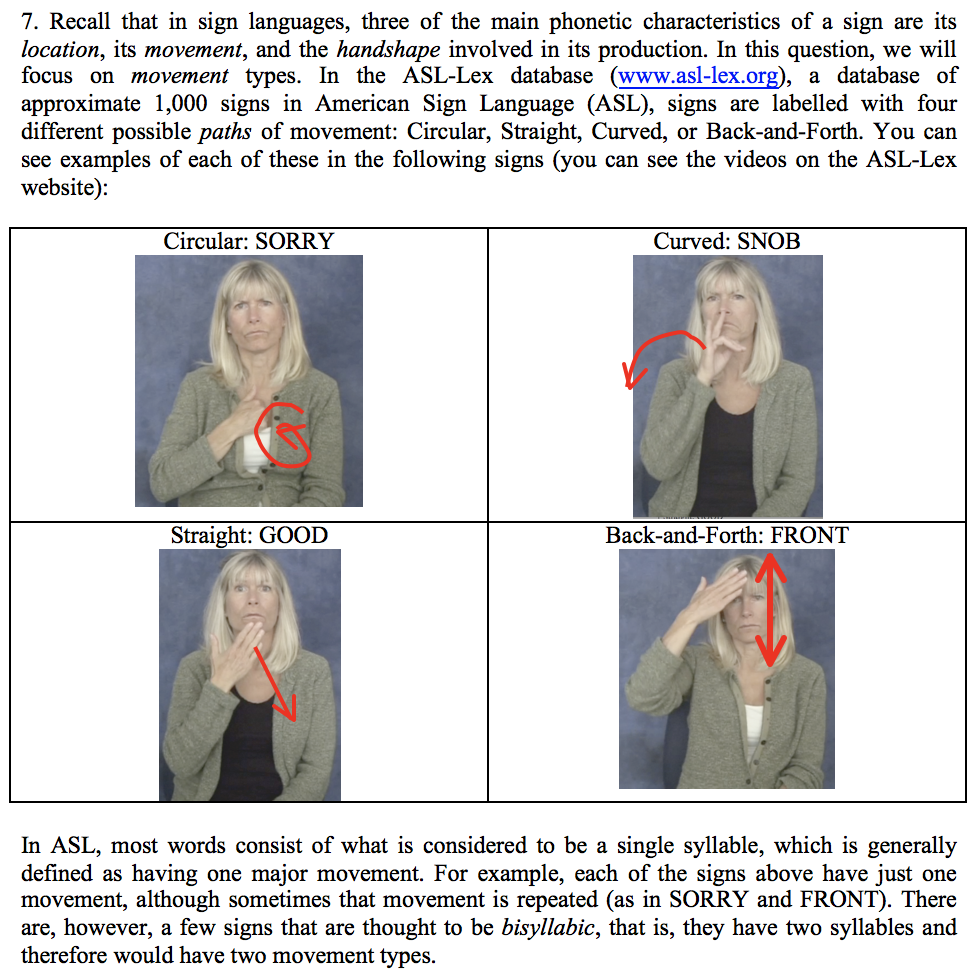
\includegraphics{../images/ASL_movement.png}
\end{figure}

\newpage

{\large Question 2}\\

Topic: Articulatory Phonetics\\
Source: Homework 1, Question 3(b)\\

Explain why this is or is not a complete phonetic natural class in standard North American English.\\

{[p]}, {[b]}


\newpage

\begin{center}
\textbf{{\color{red}{\HUGE END OF EXAM}}}\\

\end{center}
\newpage

\begin{center}
\textbf{{\color{blue}{\HUGE START OF EXAM\\}}}

\textbf{{\color{blue}{\HUGE Student ID: 50775\\}}}

\textbf{{\color{blue}{\HUGE 4:50\\}}}

\end{center}
\newpage

{\large Question 1}\\

Topic: Transcription\\
Source: Week 2 Handout, Part II\\

Is this a reasonable transcription of this word? Explain why.\\

<health>: {[hɛlð]}


\newpage

{\large Question 2}\\

Topic: Articulatory Phonetics\\
Source: Week 3 Handout, Question 13\\

Explain why this image does or does not match the description.\\

\begin{itemize} \item A two-handed sign. \item Location: In front of signer’s chin. \item Handshape: Starts with an “L” shape; index finger and thumb come together during the sign. \item Movement: Hands start crossed and then move away from each other horizontally. \end{itemize}

\begin{figure}[H]
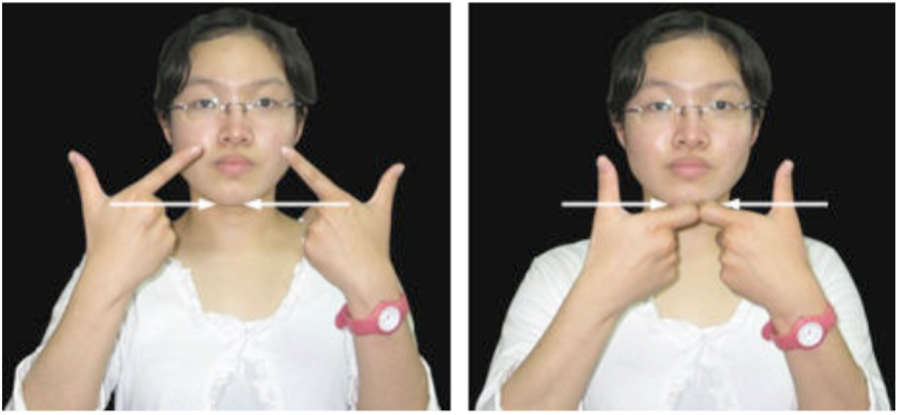
\includegraphics{../images/taiwansign_fit.png}
\caption{FIT}
\end{figure}

\newpage

\begin{center}
\textbf{{\color{red}{\HUGE END OF EXAM}}}\\

\end{center}
\newpage

\end{document}

